% \documentclass[12pt,a4paper,oneside]{report}
\documentclass[12pt,a4paper,twocolumn]{report}

% -------------------- Packages --------------------
\usepackage[utf8]{inputenc}
\usepackage[T1]{fontenc}
\usepackage{lmodern}
\usepackage{setspace}        
\usepackage{geometry}        
\geometry{margin=1in}
\usepackage{graphicx}        
\usepackage{caption}
\usepackage{subcaption}
\usepackage{amsmath,amssymb,amsthm}
\usepackage{hyperref}        
\usepackage{tocbibind}       
\usepackage{booktabs}        
\usepackage{listings}        
\usepackage{appendix}        


\usepackage{silence}
\WarningFilter{xeCJK}{Missing character}
\WarningFilter{tcolorbox}{}



% \usepackage{tcolorbox}
\usepackage[most]{tcolorbox}
\tcbuselibrary{skins}

\usepackage{fontspec} % allows direct Unicode input
\usepackage{xeCJK} % 分開設置中英文字型

\setmainfont{Times New Roman}[
Path = ./fonts/english/ ,
Extension = .ttf ,
BoldFont = *-Bold ,
ItalicFont = *-Italic ,
BoldItalicFont = *-BoldItalic, ]
\setCJKmainfont{BiauKai}[
Path = ./fonts/chinese/ ,
Extension = .ttf , ]

\usepackage{indentfirst}  % Indent first paragraph after section headings
\usepackage{enumitem}    % Customize list environments

\usepackage{titlesec}

% Set paragraph indentation
\setlength{\parindent}{0em}
% Configure lists to align with paragraph indentation
\setlist[enumerate]{leftmargin=2em, itemindent=0em}
\setlist[itemize]{leftmargin=2em, itemindent=0em}

% Format chapters - MUST be on one line or use % for line continuation
\titleformat{\chapter}[hang]{\normalfont\huge\bfseries}{\chaptertitlename\ \thechapter}{1em}{}

% Prevent chapters from starting on a new page
% \let\cleardoublepage\clearpage
\titleclass{\chapter}{straight}

% Ensure \chapter* behaves like \chapter in two-column mode
% \makeatletter
% \renewcommand{\chapter*}[1]{%
%     \if@twocolumn
%         \twocolumn[\vspace*{2cm}\centering{\huge\bfseries #1}\par\vspace{2cm}]
%         \@afterheading
%     \else
%         \par\vspace*{2cm}\centering{\huge\bfseries #1}\par\vspace{2cm}
%         \@afterheading
%     \fi
% }
% \makeatother

% Reduce space before/after chapter titles
\titlespacing*{\chapter}{0pt}{30pt}{20pt}

% \titleformat{\chapter}[hang]{\normalfont\huge\bfseries}{\chaptertitlename\ \thechapter}{1em}{}

\usepackage{caption}   % for customizing captions
\usepackage{multicol}
\usepackage{etoolbox}


% -------------------- Formatting --------------------
\onehalfspacing
\setcounter{secnumdepth}{3}
\setcounter{tocdepth}{3}

% -------------------- Helper Commands --------------------
\renewcommand{\appendix}[2]{
    \chapter*{{#1}~  ~#2}
    \phantomsection
    \addcontentsline{toc}{chapter}{{#1}~  ~#2}
    \setcounter{section}{0}
    \renewcommand{\thechapter}{#1}
}

% -------------------- Title Page --------------------
\begin{document}

% cover
\newgeometry{top=4cm, bottom=3cm, left=3cm, right=3cm}
\begin{titlepage}
    \begin{singlespace}
        \begin{center}
            % 中文校系名稱 (18, 27)
            \fontsize{18}{27}\selectfont
            國立成功大學資訊工程學系\par
            專題研究\par

            % 英文系所名稱 (14, 21)
            \fontsize{14}{21}\selectfont
            Department of Computer Science and Information Engineering\par
            College of Electrical Engineering and Computer Science\par

            % 英文學校名稱 (16, 24)
            \fontsize{16}{24}\selectfont
            National Cheng Kung University\par
            Capstone Project\par

            % 中英文論文題目 (18, 27)
            % 中英文作者姓名 (18, 27)
            % 中英文指導教授 (18, 27)
            % 論文撰寫日期   (18, 27)
            \vfill
            \fontsize{18}{27}\selectfont
            小模型,大貢獻:準確且高效的中文新聞摘要模型訓練研究\par
            Small Model, Big Impact: A Study on Training for Accurate and Efficient Chinese News Summarization Models\par
            \vfill
            王郁豪\par
            Yu-Hao Wang\par
            \vfill
            指導教授: 陳響亮 博士\par
            Advisor: Shang-Liang Chen, Ph.D.\par
            \vfill
            中華民國 114 年 6 月\par
            June, 2025
        \end{center}
    \end{singlespace}
\end{titlepage}
\clearpage
\restoregeometry

% \begin{titlepage}
%     \centering
%     \vspace*{2cm}
%     {\Huge \textbf{小模型,大貢獻:準確且高效的中文新聞摘要模型訓練研究} \par}
%     \vspace{0.5cm}
%     {\Large Small Model, Big Impact: A Study on Training for Accurate and Efficient Chinese News Summarization Models \par}
%     \vspace{2cm}
%     {\Large 指導教授:陳響亮 教授 \par}
%     {\Large 專題成員:王郁豪 \par}
%     \vfill
%     {\large 國立成功大學 資訊工程學系 \par}
%     {\large 中華民國 XXXX 年 XX 月 \par}
% \end{titlepage}

% -------------------- 前置部分 --------------------
\pagenumbering{roman}

\onecolumn
% % !TeX root = ../main.tex

\fontsize{12}{18}\selectfont

% Save the default chapter format
% \titleformat{name=\chapter,numberless}[display]
% {\normalfont\huge\bfseries}{}{0pt}{}

% Center the chapter title and make it unnumbered
% {\titleformat{name=\chapter,numberless}[display]
%    {\filcenter\normalfont\huge\bfseries}{}{0pt}{}
%  \chapter*{Acknowledgement}
%  \addcontentsline{toc}{chapter}{Acknowledgement}}

\vspace{0.65\baselineskip}
\begingroup
\let\cleardoublepage\relax
\chapter*{Acknowledgement}
\addcontentsline{toc}{chapter}{Acknowledgement}
\endgroup

I would like to express my sincere gratitude to my advisor, Professor Shang-Liang Chen, for his invaluable guidance and insightful advice throughout this research. I also thank my classmates for their thoughtful discussions and feedback, the senior lab members for their assistance in setting up the experimental environment, and an anonymous friend for providing high-end GPUs, which allowed me to perform tests and training without waiting in turn. Finally, I am deeply grateful to my family and friends for their unwavering support and encouragement throughout the course of my research.

% % !TeX root = ../main.tex

\fontsize{12}{18}\selectfont
% \chapter*{\centering Abstract}
\phantomsection
% \addcontentsline{toc}{chapter}{Abstract}


% Save the default chapter format
\titleformat{name=\chapter,numberless}[display]
{\normalfont\huge\bfseries}{}{0pt}{}

% Center the chapter title and make it unnumbered
{\titleformat{name=\chapter,numberless}[display]
   {\filcenter\normalfont\huge\bfseries}{}{0pt}{}
 \chapter*{Abstract}
 \addcontentsline{toc}{chapter}{Abstract}}

% % \begin{abstract}

In the modern era of information overload, people often lack time to read full news articles and may be influenced by sensational headlines, leading to biased understanding. This thesis develops a compact Chinese news summarization model capable of running on resource-limited devices, such as smartphones, while maintaining high comprehension and summary quality. Combining knowledge distillation and curriculum training, we compress model parameters while enhancing generalization and language understanding. A five-stage curriculum is designed to gradually teach the model traditional Chinese conversion, essential aspect extraction, reasoning construction, and summary generation. Various data generation strategies and training approaches are evaluated, including learning rate adjustments, parameter freezing, and LoRA fine-tuning. Experimental results demonstrate that a 0.5B-parameter student model achieves comparable summary quality to 3B-parameter models, outperforming similar small-scale models and generating outputs with high fluency and content coverage. This work demonstrates the feasibility of lightweight yet high-quality Chinese news summarization models and provides a practical framework for mobile deployment.

% % \end{abstract}

\twocolumn

\tableofcontents
% \listoffigures
% \listoftables
% % !TeX root = ../main.tex

% \newenvironment{denotation}[1][2.5cm]{
% \chapter*{\centering Denotation}
% \addcontentsline{toc}{chapter}{Denotation}
% \phantomsection  % Add phantom section for proper PDF bookmarks
% \noindent
% \begin{list}{}{
%   \renewcommand\makelabel[1]{\textbf{##1}\hfill}  % Make labels bold
%   \setlength{\labelwidth}{#1}                     % 符號欄寬度
%   \setlength{\labelsep}{0.5cm}                    % 標籤與列表文字距離
%   \setlength{\itemindent}{0cm}                    % 標籤縮進
%   \setlength{\leftmargin}{\labelwidth+\labelsep}  % 標籤左邊界
%   \setlength{\rightmargin}{0cm}                   % 標籤右邊界
%   \setlength{\parsep}{0cm}                        % 段落間距
%   \setlength{\itemsep}{12pt}                      % 標籤間距 (reduced for better spacing)
%   \setlength{\listparindent}{0cm}                 % 段落縮進
%   \setlength{\topsep}{12pt}                       % 標籤與上文距離 (add some space)
%   \setlength{\partopsep}{0pt}                     % Additional spacing control
% }}{\end{list}}

% Alternative simpler approach using description environment
\newenvironment{denotation}[1][2.5cm]{
  \chapter*{\centering Denotation}
  \addcontentsline{toc}{chapter}{Denotation}
  \phantomsection
  \begin{description}[leftmargin=#1,labelwidth=#1,labelsep=0.5cm,itemsep=12pt]
  \renewcommand{\makelabel}[1]{
    \hspace{0pt}\textbf{##1}\hfill
  }
}{
  \end{description}
}


\begin{denotation}[3cm]

\item[LoRA]{Low-Rank Adaptation, a technique for efficient model fine-tuning.}

\item[MLP]{Multi-Layer Perceptron, a type of feedforward neural network.}

\item[LLM]{Large Language Model, a neural network trained on vast text data for language tasks.}

\item[BERTScore]{BERT-based Text Similarity Evaluation, a metric for comparing text using BERT embeddings.}

\item[ROUGE]{Recall-Oriented Understudy for Gisting Evaluation, a set of metrics for automatic text summarization evaluation.}

\item[B-F1]{F1 score of BERTScore, measuring text similarity.}

\item[R-1]{ROUGE-1 F1 score, based on unigram overlap.}

\item[R-2]{ROUGE-2 F1 score, based on bigram overlap.}

\item[R-L]{ROUGE-L F1 score, based on the longest common subsequence.}

\item[R-Lsum]{ROUGE-Lsum F1 score, for summary-level evaluation using longest common subsequence.}

\item[Judge]{Combined score for naturalness and information coverage, evaluated by a teacher model.}

\item[Qwen]{Qwen, a Chinese large language model developed by Alibaba Cloud.}

\item[Gemma]{Gemma, a large language model developed by Google.}

\item[PEFT]{Parameter-Efficient Fine-Tuning, a method for adapting models with fewer parameters.}

\item[GPU]{Graphics Processing Unit, hardware for parallel computation.}

\item[CPU]{Central Processing Unit, the main processor of a computer.}

\item[API]{Application Programming Interface, a set of protocols for building software applications.}

\item[JSON]{JavaScript Object Notation, a lightweight data-interchange format.}

\item[NLP]{Natural Language Processing, the field of processing and analyzing human language.}

\item[AI]{Artificial Intelligence, the simulation of human intelligence by machines.}

\end{denotation}
            % 符號列表(Denotation)

% --------------- Contents of Thesis ---------------
% \mainmatter
\clearpage
\pagenumbering{arabic}

% \setlength{\parindent}{2em}

% \titleformat{\chapter}[hang]
%   {\normalfont\huge\bfseries} % format
%   {\thechapter}               % only number
%   {1em}                       % spacing
%   {}  

% \let\cleardoublepage\clearpage

% --- Chapter style ---
\titleformat{\chapter}[hang]
  {\large\bfseries}         % Font
  {\thechapter.}{0.5em}{}   % Numbering style
\titlespacing*{\chapter}{0pt}{0pt}{6pt} 
% {left}{before}{after}

% Ensure \chapter* uses the same style as numbered chapters
\titleformat{name=\chapter,numberless}[hang]
    {\large\bfseries}
    {}{0pt}{}
\titlespacing*{name=\chapter,numberless}{0pt}{0pt}{6pt}

% --- Section style ---
\titleformat{\section}[hang]
  {\normalsize\bfseries}
  {\thesection}{0.5em}{}
\titlespacing*{\section}{0pt}{4pt}{4pt}


% 控制 caption 與表格之間的距離
\captionsetup[table]{skip=5pt} % 預設大約 10pt, 改小一點
\captionsetup[figure]{skip=5pt}

% \setlength{\belowcaptionskip}{-15pt}
% \setlength{\textfloatsep}{180pt} % 控制浮動表格與正文的距離
% \setlength{\floatsep}{120pt}     % 控制兩個浮動體之間的距離

% Reduce font size for all tables

\AtBeginEnvironment{table}{\small}


\newpage
% \twocolumn
% \begin{multicols}{2}
% % !TeX root = ../main.tex

\chapter{Introduction}

\section{Motivation}
In today’s fast-paced society, the public often lacks the time to thoroughly read complete news articles. Sensational headlines may bias information judgment. A compact Chinese summarization model capable of running on mobile devices could efficiently provide concise and meaningful summaries, improving both the speed and quality of information acquisition.

\section{Objectives}

The goal of this research is to combine knowledge distillation and curriculum training strategies to compress model parameters while enhancing generalization and language comprehension. The ultimate aim is to deploy a high-quality Chinese news summarization system on mobile devices, achieving a small-model, high-quality solution.

% !TeX root = ../main.tex

\chapter{Methodology}
\section{Data Collection}
To construct the training corpus, a web crawler was implemented to collect news articles from \textit{United Daily News}. In addition, the YeungNLP/firefly-pretrain-dataset was incorporated as supplementary pretraining data. This combination provided both domain-specific content and a broader linguistic foundation for model development.

\section{Model Selection}
Two models from the Qwen2.5 family were adopted. The student model was Qwen2.5-0.5B-Instruct, a lightweight 0.5-billion-parameter model intended for efficient training and deployment. The teacher model was Qwen2.5-32B-Instruct, which was used not only to generate synthetic training data but also to provide preprocessing guidance and evaluation signals during experimentation.

\section{Curriculum Training}
The training process was organized into five progressive stages (S1–S5) designed to gradually increase task complexity. First, traditional Chinese text was standardized using OpenCC (S1). Next, essential aspects were extracted from each article (S2), followed by the construction of reasoning triples that captured semantic relationships among these aspects (S3). Building on this foundation, the model then generated summaries based on the content together with the extracted aspects and triples (S4). Finally, the most challenging stage required the model to generate summaries directly from the raw news content (S5).

\section{Data Generation Strategies}
Different strategies were explored to generate training data. The \textbf{V1 strategy} relied on a single step to jointly produce aspects, triples, and summaries. \textbf{V2} followed a sequential approach in which aspects were first generated, then expanded into triples, and finally used to construct summaries. \textbf{V3} reversed the order by generating the summary first and subsequently deriving aspects and triples from it. \textbf{V4} extended V3 with manual corrections to reduce noise and improve training quality. The final dataset was divided into 23,848 training articles, 5,960 validation articles, and 6,052 test articles, as summarized in Table~\ref{tab:dataset_statistics}.

{
    \captionof{table}{Dataset Statistics}
    \label{tab:dataset_statistics}
    \centering
    \resizebox{\columnwidth}{!}{
    \begin{tabular}{lccc}
        \toprule
        Dataset & Training & Validation & Testing \\
        \midrule
        Number of articles & 23848 & 5960 & 6052 \\
        \bottomrule
    \end{tabular}}
}

\section{Training Strategies}
Several fine-tuning strategies were evaluated. The default configuration applied a decaying learning rate. A variant, denoted \texttt{lr\_adj}, maintained a constant learning rate in Stage 5 to prevent premature convergence. Other experiments selectively froze model components, either keeping only attention layers (\texttt{only\_attn}) or only MLP layers (\texttt{only\_mlp}) trainable, to measure their relative contributions. LoRA-based adaptation was also tested, applying low-rank factorization to MLP (rank 160) and attention (rank 32) layers. Finally, combinations of these methods were explored to assess possible synergies.

\section{Evaluation Metrics}
Model outputs were evaluated using both automatic and human-aligned metrics. ROUGE-1, ROUGE-2, and ROUGE-L were applied to measure n-gram overlap with reference summaries, while BERTScore was used to capture semantic similarity. In addition, the teacher model (32B) was employed as a judge to assess naturalness and information coverage, providing a complementary qualitative evaluation beyond automatic metrics.

% !TeX root = ../main.tex

\setlength{\parindent}{0em}
\chapter{Experiments}
\section{Data Generation Strategy Comparison}
The first set of experiments focused on evaluating different strategies for generating training data, with the goal of identifying which approach most effectively facilitates downstream summarization. Direct reasoning (V1), in which the teacher model was required to infer key elements and triples before producing the summary, consistently produced incomplete and incoherent outputs. Although some degree of logical consistency was maintained, the generated summaries often lacked sufficient coverage of important content, limiting their utility as high-quality training data.

An alternative stage-by-stage strategy (V2) was designed to mitigate these issues by splitting the generation process into multiple steps. Contrary to expectation, however, this approach worsened coherence and frequently led to “out-of-focus” summaries in which the generated key elements diverged substantially from the final summaries. This indicates that decomposing the generation into smaller stages can actually amplify inconsistencies, making it difficult for the student model to learn meaningful reasoning patterns.

In contrast, the summary-first strategy (V3) demonstrated clear advantages. By first producing a coherent summary and then deriving supporting elements and triples, this method yielded the highest performance across all automatic and human-aligned evaluation metrics, including ROUGE, BERTScore, and Judge scores. These results suggest that ensuring coherence at the summary level provides a stable foundation for subsequent reasoning tasks, which in turn improves both training efficiency and output quality. Table~\ref{tab:strategy_comparison} presents the quantitative comparison of the three strategies.

\begin{center}
    \captionof{table}{Performance Comparison by Data Generation Strategy}
    \label{tab:strategy_comparison}
    \resizebox{\columnwidth}{!}{
    \begin{tabular}{lccccc}
        \toprule
        Model & R-1 & B-F1 & Judge & R-2 & R-L \\
        \midrule
        4stg\_v3 & \textbf{45.5} & \textbf{77.9} & \textbf{70.3} & \textbf{24.3} & \textbf{37.6} \\
        4stg\_v1 & 43.8 & 76.8 & 64.0 & 22.1 & 35.5 \\
        4stg\_v2 & 37.6 & 69.4 & 65.1 & 17.5 & 23.4 \\
        \bottomrule
    \end{tabular}}
\end{center}

\section{Training Strategy Comparison}
The second set of experiments explored alternative training strategies, with particular attention to learning rate schedules and parameter-freezing techniques. A key finding was that adopting a non-decaying learning rate significantly improved model performance. This suggests that, unlike larger-scale models where decay is often beneficial to avoid overfitting, smaller student models benefit from maintaining a steady learning signal throughout training.
Another observation concerns the role of different parameter groups. Freezing only the attention layers or only the MLP layers still resulted in relatively strong performance, indicating that both components of the network contribute meaningfully to summarization ability. For example, the ``only\_mlp'' variant retained a high BERTScore (78.6\%), suggesting that attention-driven representations alone can sustain semantic fidelity.

By contrast, the application of LoRA, though successful in other low-resource fine-tuning scenarios, failed to provide improvements in this summarization setting. In fact, performance stagnated or slightly regressed. This result not only underscores the task-specific nature of parameter-efficient methods but also highlights a potential conflict between LoRA’s parameter expansion and the principle of maintaining a lightweight student model. The results of these comparisons are reported in Table~\ref{tab:training_strategy_comparison}.

{
    \captionof{table}{Performance Comparison by Training Strategy}
    \label{tab:training_strategy_comparison}
    \centering
    \resizebox{\columnwidth}{!}{
    \begin{tabular}{lccccc}
        \toprule
        Model & R-1 & B-F1 & Judge & R-2 & R-L \\
        \midrule
        4stg\_v3-lr\_adj & \textbf{48.4} & \textbf{79.3} & 72.8 & \textbf{25.7} & \textbf{40.1} \\
        4stg\_v3-lr\_adj-only\_mlp & 46.6 & 78.6 & 71.5 & 24.2 & 38.4 \\
        4stg\_v3-lr\_adj\_lora & 45.6 & 78.0 & \textbf{73.6} & 23.3 & 37.4 \\
        4stg\_v3 & 45.5 & 77.9 & 70.3 & 24.3 & 37.6 \\
        4stg\_v3-lr\_adj-only\_attn & 45.2 & 77.8 & 69.1 & 23.0 & 37.1 \\
        \bottomrule
    \end{tabular}}
}

\section{Curriculum Stage Comparison}
The final set of experiments investigated the influence of curriculum learning, particularly the number of curriculum stages, on model performance. The findings reveal a nuanced picture. When trained without a decaying learning rate, models with a single stage occasionally achieved marginally higher ROUGE-1 scores compared to those trained with multiple stages. However, multi-stage setups (four or five stages) consistently yielded more accurate Traditional Chinese generation and greater stability in output quality. This suggests that while curriculum depth may not always maximize surface-level evaluation scores, it enhances the stylistic fidelity and robustness of the generated summaries.
Tables~\ref{tab:stage_lr_decay}--\ref{tab:stage_no_lr_decay} summarize these results, and Figure~\ref{fig:zh_tw_result} illustrates the proportion of Traditional Chinese in outputs among different models, especially in terms of improvements.

% \begin{table}[ht]
%     \centering
%     \caption{Performance of Different Stage Numbers with Decaying Learning Rate}
%     \begin{tabular}{lccccc}
%         \toprule
%         MODEL & R-1 & B-F1 & Judge & R-2 & R-L \\
%         \midrule
%         Qwen2.5-0.5B\_4stg\_v3 & 45.5 & \textbf{77.9} & \textbf{70.3} & \textbf{24.3} & 37.6 \\
%         Qwen2.5-0.5B\_1stg\_v3 & \textbf{45.9} & 77.9 & 68.8 & 23.7 & \textbf{37.7} \\
%         \bottomrule
%     \end{tabular}
%     \label{tab:stage_lr_decay}
% \end{table}

% \begin{table}[ht]
%     \centering
%     \caption{Performance of Different Stage Numbers without Decaying Learning Rate}
%     \begin{tabular}{lccccc}
%         \toprule
%         MODEL & R-1 & B-F1 & Judge & R-2 & R-L \\
%         \midrule
%         Qwen2.5-0.5B\_1stg\_v4-lr\_adj & \textbf{47.0} & \textbf{78.8} & \textbf{75.9} & \textbf{24.5} & \textbf{38.9} \\
%         Qwen2.5-0.5B\_4stg\_v4-lr\_adj & 46.8 & 78.6 & 75.2 & 24.2 & 38.6 \\
%         Qwen2.5-0.5B\_5stg\_v4-lr\_adj & 46.5 & 78.6 & 75.1 & 23.9 & 38.3 \\
%         \bottomrule
%     \end{tabular}
%     \label{tab:stage_no_lr_decay}
% \end{table}

% \begin{figure}[htbp]  % h=here, t=top, b=bottom, p=page of floats
%     \centering
%     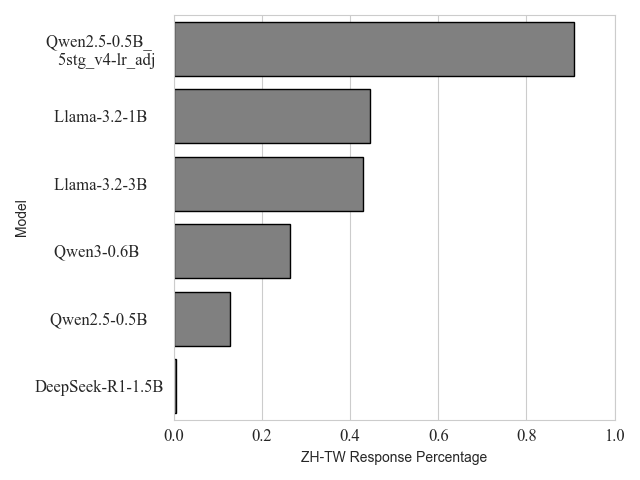
\includegraphics[width=0.7\textwidth]{figures/zh_tw_result_percentage_overall.png}
%     \caption{Proportion of Traditional Chinese responses generated by each model. The proposed 0.5B model with 5-stage curriculum achieves the highest ratio, surpassing even 3B models.}
%     \label{fig:zh_tw_result}
% \end{figure}

\vspace{0.75\baselineskip}
{
    \captionof{table}{Performance Comparison by Training Strategy}
    \label{tab:training_strategy_comparison}
    \centering
    \resizebox{\columnwidth}{!}{
    \begin{tabular}{lccccc}
        \toprule
        Model & R-1 & B-F1 & Judge & R-2 & R-L \\
        \midrule
        4stg\_v3-lr\_adj & \textbf{48.4} & \textbf{79.3} & 72.8 & \textbf{25.7} & \textbf{40.1} \\
        4stg\_v3-lr\_adj-only\_mlp & 46.6 & 78.6 & 71.5 & 24.2 & 38.4 \\
        4stg\_v3-lr\_adj\_lora & 45.6 & 78.0 & \textbf{73.6} & 23.3 & 37.4 \\
        4stg\_v3 & 45.5 & 77.9 & 70.3 & 24.3 & 37.6 \\
        4stg\_v3-lr\_adj-only\_attn & 45.2 & 77.8 & 69.1 & 23.0 & 37.1 \\
        \bottomrule
    \end{tabular}}
    \vspace{0.75\baselineskip}
}

% ------------------ TABLE 2.4 ------------------
{
    \captionof{table}{Performance of Different Stage Numbers with Decaying Learning Rate}
    \label{tab:stage_lr_decay}
    \centering
    \resizebox{\columnwidth}{!}{
    \begin{tabular}{lccccc}
        \toprule
        Model & R-1 & B-F1 & Judge & R-2 & R-L \\
        \midrule
        Qwen2.5-0.5B\_4stg\_v3 & 45.5 & \textbf{77.9} & \textbf{70.3} & \textbf{24.3} & 37.6 \\
        Qwen2.5-0.5B\_1stg\_v3 & \textbf{45.9} & 77.9 & 68.8 & 23.7 & \textbf{37.7} \\
        \bottomrule
    \end{tabular}}
}
\vspace{0.75\baselineskip}
\vspace{0.75\baselineskip}

% \begin{center}
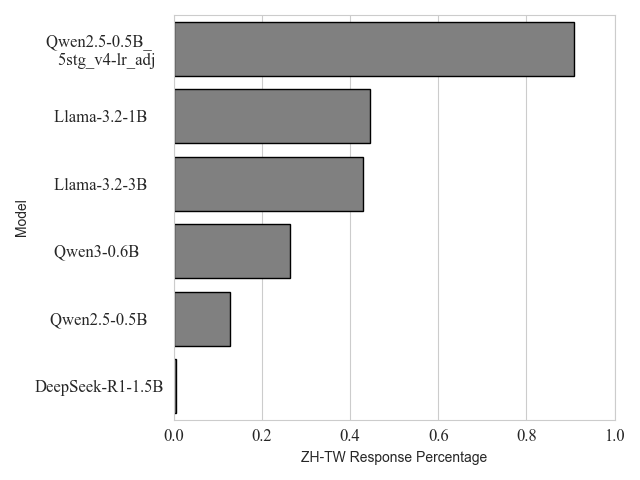
\includegraphics[width=\columnwidth]{figures/zh_tw_result_percentage_overall.png}
\captionof{figure}{Proportion of Traditional Chinese responses generated by each model. The proposed 0.5B model with 5-stage curriculum achieves the highest ratio, surpassing even 3B models.}
\label{fig:zh_tw_result}
% \end{center}

Furthermore, the benefits of curriculum learning appeared to depend heavily on the scale of pretraining. When large-scale pretraining was employed, curriculum learning only slightly improved summary quality. In contrast, with smaller pretraining datasets, curriculum learning provided substantial performance boosts, indicating that staged training helps compensate for weaker initial representations by guiding the model through progressively more complex tasks. As shown in Table~\ref{tab:custom_pretrain_stage_comparison}, the 4-stage curriculum model (Custom-pretrained-4stg\_v3-lr\_adj) consistently outperforms the single-stage counterpart across most metrics, particularly in ROUGE-1 and Judge scores, highlighting the effectiveness of gradual task progression in low-resource pretraining scenarios.

% \begin{table}[ht]
%     \centering
%     \caption{Performance of Custom Pretrained Models with Different Curriculum Stages}
%     \begin{tabular}{lccccc}
%         \toprule
%         Model & R-1 & B-F1 & Judge & R-2 & R-L \\
%         \midrule
%         Custom-pretrained-4stg\_v3-lr\_adj & \textbf{13.3} & \textbf{50.6} & \textbf{0.9} & \textbf{1.8} & 4.0 \\
%         Custom-pretrained-1stg\_v3-lr\_adj & 11.8 & 50.5 & 0.6 & 1.5 & \textbf{5.0} \\
%         \bottomrule
%     \end{tabular}
%     \label{tab:custom_pretrain_stage_comparison}
% \end{table}


% ------------------ TABLE 2.5 ------------------
{
    \captionof{table}{Performance of Different Stage Numbers without Decaying Learning Rate}
    \label{tab:stage_no_lr_decay}
    \centering
    \resizebox{\columnwidth}{!}{
    \begin{tabular}{lccccc}
        \toprule
        Model & R-1 & B-F1 & Judge & R-2 & R-L \\
        \midrule
        Qwen2.5-0.5B\_1stg\_v4-lr\_adj & \textbf{47.0} & \textbf{78.8} & \textbf{75.9} & \textbf{24.5} & \textbf{38.9} \\
        Qwen2.5-0.5B\_4stg\_v4-lr\_adj & 46.8 & 78.6 & 75.2 & 24.2 & 38.6 \\
        Qwen2.5-0.5B\_5stg\_v4-lr\_adj & 46.5 & 78.6 & 75.1 & 23.9 & 38.3 \\
        \bottomrule
    \end{tabular}}
}


% !TeX root = ../main.tex

\chapter{Results}

\section{Final Model Performance}
The final 0.5B model achieves performance approaching that of larger 3B models in ROUGE-1 and BERTScore, demonstrating substantial improvements in summary generation quality. It significantly outperforms comparable small models, such as the Gemma series, with ROUGE-1 gains of approximately 5–7\%, reaching a practically usable level. Compared with its pre-trained version before post-training and curriculum stages, the model’s Judge score increased by over 0.16, indicating that the training strategy effectively enhanced the naturalness and informativeness of generated summaries.

Table~\ref{tab:final_05B_comparison} shows a comparison of the final 0.5B model with other models of similar parameter scale and larger teacher models. The results suggest that careful curriculum training allows smaller models to approach the performance of significantly larger ones, closing the gap in both automatic evaluation metrics and human-judged quality.

% \begin{table}[ht]
%   \centering
%   \caption{Performance Comparison of Final 0.5B Model with Other Models of Similar Parameter Scale}

\begin{center}
    \captionof{table}{Performance Comparison of Final 0.5 Model with Other Models of Similar Parameter Scale}
    \label{tab:final_05B_comparison}
    \resizebox{\columnwidth}{!}{
    \begin{tabular}{lccccc}
    \toprule
    Model & R-1 & B-F1 & Judge & R-2 & R-L \\
    \midrule
    Qwen2.5-32B & \textbf{55.6} & \textbf{82.2} & 81.7 & \textbf{34.9} & \textbf{48.2} \\
    Qwen2.5-3B & 49.5 & 79.8 & \textbf{83.8} & 26.2 & 40.1 \\
    Qwen2.5-0.5B\_5stg\_v4-lr\_adj & 46.5 & 78.6 & 75.1 & 23.9 & 38.3 \\
    Llama-3.2-3B & 43.3 & 76.8 & 74.3 & 20.7 & 34.7 \\
    Gemma-3-1B & 41.8 & 76.0 & 72.6 & 18.3 & 31.2 \\
    Qwen2.5-0.5B & 39.7 & 74.8 & 58.7 & 18.5 & 30.9 \\
    Gemma-2-2B & 39.3 & 71.9 & 83.4 & 18.3 & 26.2 \\
    Llama-3.2-1B & 38.7 & 74.1 & 63.4 & 16.9 & 29.5 \\
    DeepSeek-R1-1.5B & 32.2 & 71.3 & 65.8 & 12.0 & 21.4 \\
    \bottomrule
    \end{tabular}}
\end{center}
% \end{table}

\section{Traditional Chinese Generation}
In addition to overall performance, the model demonstrates marked improvements in linguistic handling. After post-training, the proportion of Traditional Chinese output rises significantly, even exceeding that of the teacher model. The percentage of responses completely free of Simplified Chinese characters is also higher than in other models, highlighting the effectiveness of the training data and curriculum strategy in producing culturally and linguistically appropriate text.

\section{Mitigation of Teacher Model Errors}
Beyond linguistic improvements, the model also mitigates issues inherited from the teacher model. Quantitative analysis shows that abnormal or unexpected endings are fully corrected: among 30,296 samples, 2,871 instances contained irregular endings (e.g., “\texttt{\textbackslash n hổ \textbackslash n}”) in the teacher model, whereas after post-training, none of these anomalies appeared. This demonstrates that the staged curriculum learning and high-quality training dataset effectively addressed imperfections present in the original teacher outputs.
% !TeX root = ../main.tex

\chapter{Conclusion}

This study systematically explored strategies for building lightweight Chinese summarization models, focusing on data generation, training configurations, and curriculum learning. The results provide both methodological insights and practical guidance for the development of efficient yet high-quality summarization systems.

In terms of \textbf{data generation}, the experiments reveal that direct reasoning and stage-by-stage decomposition tend to produce incomplete or unfocused outputs, limiting their usefulness as training data. By contrast, a \textbf{summary-first approach} consistently delivers coherent and comprehensive summaries, establishing a stable foundation for downstream reasoning and enabling more effective student–teacher distillation.

Regarding \textbf{training strategies}, a \textbf{non-decaying learning rate combined with full parameter fine-tuning} outperforms methods such as LoRA and partial freezing, indicating that full fine-tuning remains the most effective choice. Moreover, contrary to expectations, LoRA and partial freezing provide little benefit in terms of training time or VRAM savings, further reinforcing the practicality of full parameter fine-tuning.

The investigation of \textbf{curriculum learning} further highlights its importance in low-resource conditions. While multi-stage curricula contribute modest gains when large-scale pretraining is available, they prove highly effective for smaller, custom-pretrained models, substantially improving summarization accuracy, stylistic fidelity, and robustness. This staged progression also enables the student model to mitigate errors inherited from the teacher, such as abnormal token sequences and inconsistent linguistic output.

Taken together, these strategies enabled the development of a \textbf{0.5B-parameter model} that approaches the performance of much larger 3B models, while outperforming comparable small-scale baselines. Notably, the model demonstrates strong handling of Traditional Chinese, surpassing even its teacher in linguistic appropriateness.

In conclusion, this work demonstrates that through \textbf{summary-first data generation, full fine-tuning with steady learning signals, and curriculum-based task progression}, it is possible to achieve a balance of \textbf{efficiency, robustness, and high-quality summarization} within a compact architecture. The proposed framework not only advances the practical deployment of lightweight summarization models, including mobile applications, but also provides a replicable pathway for future research on resource-efficient natural language processing.


% -------------------- Back Matter --------------------
% !TeX root = ../main.tex

\fontsize{12}{18}\selectfont

% Save the default chapter format
% \titleformat{name=\chapter,numberless}[display]
% {\normalfont\huge\bfseries}{}{0pt}{}

% Center the chapter title and make it unnumbered
% {\titleformat{name=\chapter,numberless}[display]
%    {\filcenter\normalfont\huge\bfseries}{}{0pt}{}
%  \chapter*{Acknowledgement}
%  \addcontentsline{toc}{chapter}{Acknowledgement}}

\vspace{0.65\baselineskip}
\begingroup
\let\cleardoublepage\relax
\chapter*{Acknowledgement}
\addcontentsline{toc}{chapter}{Acknowledgement}
\endgroup

I would like to express my sincere gratitude to my advisor, Professor Shang-Liang Chen, for his invaluable guidance and insightful advice throughout this research. I also thank my classmates for their thoughtful discussions and feedback, the senior lab members for their assistance in setting up the experimental environment, and an anonymous friend for providing high-end GPUs, which allowed me to perform tests and training without waiting in turn. Finally, I am deeply grateful to my family and friends for their unwavering support and encouragement throughout the course of my research.

\clearpage

% -------------------- References --------------------

\renewcommand{\bibname}{References}

\begin{thebibliography}{99}

\bibitem{vaswani2017a} Ashish Vaswani, Noam Shazeer, Niki Parmar, Jakob Uszkoreit, Llion Jones, Aidan N Gomez, Łukasz Kaiser, and Illia Polosukhin. (2017a). Attention is all you need. In Advances in Neural Information Processing Systems, volume 30. Curran Associates, Inc.

\bibitem{vaswani2017b} Ashish Vaswani, Noam Shazeer, Niki Parmar, Jakob Uszkoreit, Llion Jones, Aidan N Gomez, Łukasz Kaiser, and Illia Polosukhin. (2017b). Attention is all you need. Advances in neural information processing systems, 30.

\bibitem{trisum} Pengcheng Jiang, Cao Xiao, Zifeng Wang, Parminder Bhatia, Jimeng Sun, Jiawei Han. (2024). TriSum: Learning Summarization Ability from Large Language Models with Structured Rationale. arXiv preprint arXiv:2403.10351.

\bibitem{lora} Edward J. Hu, Yelong Shen, Phillip Wallis, Zeyuan Allen-Zhu, Yuanzhi Li, Shean Wang, Lu Wang, Weizhu Chen. (2021). LoRA: Low-Rank Adaptation of Large Language Models. arXiv preprint arXiv:2106.09685.

\end{thebibliography}

% \cleardoublepage
% \phantomsection
% \renewcommand{\bibname}{References}
% \addcontentsline{toc}{chapter}{References}
% \bibliographystyle{abbrv}
% \bibliography{back/references}


% -------------------- Appendices --------------------

% Revert chapter style to start on a new page (default behavior)
\titleclass{\chapter}{top}
% \end{multicols}
% % !TeX root = ../main.tex

% This could be moved to acknowledgments or conclusion instead
% But if kept as appendix, here's a better format:

\appendix{A}{Source Code and Implementation}

本研究的完整實作代碼、實驗數據以及模型配置檔案已開源發布,可透過以下連結取得:

\bigskip
\noindent \textbf{GitHub Repository:} \\
\url{https://github.com/BennyWang1007/Individual-studies}

\bigskip
\noindent 儲存庫包含:
\begin{itemize}
\item 模型訓練與微調腳本
\item 數據預處理工具
\item 實驗配置文件
\item 評估指標計算程式
\item 模型推理與部署代碼
\end{itemize}

% !TeX root = ../main.tex

% Define font size variables for tcolorbox titles and content
\newcommand{\promptTitleFontSize}{\small}
\newcommand{\promptContentFontSize}{\fontsize{8pt}{10pt}\selectfont}

\tcbset{
  promptstyle/.style={
    boxrule=0.8pt,
    arc=4mm,
    top=3mm,
    bottom=3mm,
    left=3mm,
    right=3mm,
    fonttitle=\bfseries,
    % breakable,
    fonttitle=\promptTitleFontSize, fontupper=\promptContentFontSize
  }
}

\onecolumn

\appendix{A}{Prompt Templates and Examples}

This appendix provides the prompt templates and examples used in this study, including the complete prompt designs for different versions of essential aspect extraction, triple generation, summary generation, and model evaluation.

% V1 prompt
\begin{tcolorbox}[promptstyle, title=Prompt for generating V1 summary with essential aspects and triples]
System prompt:\newline
給定一份文章,完成以下任務:\newline
(1) 提取新聞的關鍵要素,關鍵要素應為關鍵短句、名詞或事實。\newline
(2) 對於每個關鍵要素,檢索詳細的三元組,格式為 [實體1 | 關係 | 實體2],這些三元組用於構成摘要。\newline
(3) 使用檢索到的三元組撰寫一份摘要。\newline
核心要素、三元組和撰寫的摘要應該在同一份回應中,並以換行符分隔。所有三元組 [實體1 | 關係 | 實體2] 的長度必須為3(以 "|" 分隔)。\newline
範例:\newline
================範例=================\newline
提示:\newline
新聞:\newline
\{新聞\} \newline
\newline
更新:\newline
核心要素: \newline
[關鍵要素1]、[關鍵要素2]、[關鍵要素3]、...\newline
\newline
三元組:\newline
[實體1\_1 | 關係\_1 | 實體1\_2]\newline
[實體2\_1 | 關係\_2 | 實體2\_2]\newline
[實體3\_1 | 關係\_3 | 實體3\_2]\newline
...\newline
\newline
生成摘要:\newline
\{摘要\}\newline

=============================================================================================\newline
User prompt:\newline
新聞:\newline\{news\}
\end{tcolorbox}

% Example of arranging multiple tcolorboxes
\noindent
% \begin{minipage}[t]{0.48\textwidth}
\begin{tcolorbox}[promptstyle, title=Prompt for generating V2 essential aspects]
System prompt:\newline
請根據以下新聞內容,提取新聞的關鍵要素,關鍵要素應為關鍵短句、名詞或事實,請用中文回答,並且不要使用任何標點符號。請將每個關鍵要素用[]與、分隔。例如:\newline
關鍵要素:\newline
[關鍵要素1]、[關鍵要素2]、[關鍵要素3]\newline
=============================================================================================\newline
User prompt:\newline
新聞:\newline
\{news\}
\end{tcolorbox}
% \end{minipage}
% \hfill
% \begin{minipage}[t]{0.48\textwidth}
\begin{tcolorbox}[promptstyle, title=Prompt for generating V2 triples, fonttitle=\promptTitleFontSize, fontupper=\promptContentFontSize]
System prompt:\newline
請根據以下新聞內容與關鍵要素,檢索詳細的三元組,格式為 [實體1 | 關係 | 實體2],這些三元組用於構成摘要,請用中文回答,並且不要使用任何標點符號。所有三元組用[]與、分隔,且長度必須為3。\newline
例如:\newline
三元組:\newline
[實體1\_1 | 關係\_1 | 實體1\_2]、[實體2\_1 | 關係\_2 | 實體2\_2]、...\newline
=============================================================================================\newline
User prompt:\newline
新聞:\newline
\{news\}\newline

關鍵要素:\newline
\{essential\_aspects\}
\end{tcolorbox}
% \end{minipage}

\vspace{3mm} % space between rows
\noindent
% \begin{minipage}[t]{0.98\textwidth}
\begin{tcolorbox}[promptstyle, title={Prompt for generating V2 summary}]
System prompt:\newline
請根據以下新聞內容與檢索到的關鍵要素以及三元組,為新聞生成一份摘要,請用繁體中文回答。\newline
例如:\newline
生成摘要:\newline
=============================================================================================\newline
User prompt:\newline
新聞:\newline
\{news\}\newline
\newline
關鍵要素:\newline
\{essential\_aspects\}\newline

三元組:\newline
\{triples\}
\end{tcolorbox}
% \end{minipage}

\vspace{3mm}
\noindent
% \begin{minipage}[t]{0.98\textwidth}
\begin{tcolorbox}[promptstyle, title={Prompt for generating V3 summary}]
System prompt:\newline
請根據以下新聞內容,為新聞生成一份100字內精簡的摘要,請用繁體中文回答。\newline
例如:\newline
生成摘要:\newline

User prompt:\newline
新聞:\newline
\{news\}
\end{tcolorbox}
% \end{minipage}

\vspace{3mm}
\noindent
% \begin{minipage}[t]{0.98\textwidth}
\begin{tcolorbox}[promptstyle, title={Prompt for generating V3 essential aspects and triples}, fonttitle=\promptTitleFontSize, fontupper=\promptContentFontSize]
System prompt:\newline
請根據以下新聞內容以及摘要,提取新聞的關鍵要素與三元組,關鍵要素應為關鍵短句、名詞或事實,三元組應為[實體1 | 關係 | 實體2]的格式,這些三元組用於構成摘要,請用繁體中文回答。請將每個關鍵要素與三元組用[]與、分隔。例如:\newline
關鍵要素:\newline
[關鍵要素1]、[關鍵要素2]、[關鍵要素3]、...\newline
\newline
三元組:\newline
[實體1\_1 | 關係\_1 | 實體1\_2]、[實體2\_1 | 關係\_2 | 實體2\_2]、...\newline
\newline
User prompt:\newline
新聞:\newline
\{news\}\newline

摘要:\newline
\{summary\}
\end{tcolorbox}
% \end{minipage}

\vspace{3mm}
\noindent
% \begin{minipage}[t]{0.98\textwidth}
\begin{tcolorbox}[promptstyle, title={Example news, essential aspects, triples, and summary (V3)}]
新聞:\newline
母愛不分物種。動保組織接獲民眾通報發現草叢有一窩胖嘟嘟奶汪,沒想到牠們的母親為了照顧這些孩子把自己餓成皮包骨,還有嚴重營養不良跟脫水狀況,對比起小狗們都肥碩健康,狗媽媽更是令人心疼。\newline
根據The Dodo報導,美國密蘇里州(Missouri)聖路易斯流浪動物救援組織(Stray Rescue of St. Louis,SRSL)日前接獲民眾通報,說草叢裡面發現一窩肥胖的奶汪,但卻找不到狗媽媽,希望他們可以派人來協助一下。動物救援組織工作人員湯姆森(Natalie Thomson)表示,當他們趕往民眾通報的現場,的確真的看到一窩被照顧得好好的奶汪,很像是被人飼養後遺棄在附近。\newline
但令動保人員意外的一幕出現了,他們過沒多久在附近的草叢找到了狗媽媽,可是這隻渾身骨瘦如柴、幾乎可以用皮包骨形容的黃狗顯然非常營養不良,跟牠一窩肥壯幼崽形成強烈對比,這隻狗媽媽顯得有些害怕人類,但牠並沒有逃跑或是圖保護孩子,反而是將目光投射在小狗身上,希望眼前的人類不要傷害牠的孩子。\newline
每一隻狗寶寶都相當健康可愛甚至還有點肥。 (圖/取自Stray Rescue of St. Louis官網)\newline
後來這一窩共10隻奶汪跟牠們孱弱的母親都被聖路易斯流浪動物救援組織帶回收容所,經過健康檢查後反而讓獸醫跟動保人員更難過了,因為這10隻小奶狗除了有點寄生蟲問題之外,沒有任何營養不良的狀況,甚至還有些過重,但狗媽媽卻嚴重營養不良還脫水,可以說為了照顧孩子鞠躬盡瘁。\newline
目前這一窩小奶汪都受到良好的照顧,不日將可開放認養,而狗媽媽則因為身體虛弱還需要靜養一段時間才可以考慮出養。湯姆森說,這隻狗媽媽其實是很溫柔的,只是個性比較慢熟,所以需要有愛心跟耐心的飼主陪伴,牠就會慢慢敞開心房願意相信人類。\newline
\newline
摘要:\newline
美國密蘇裡州一窩小狗被發現肥胖健康,但牠們的母親卻因照顧孩子而嚴重營養不良、脫水。這11隻狗已被救出,小狗們即將開放認養,母親則需繼續靜養。救援組織尋找有耐心的飼主,以陪伴這位溫柔但慢熟的母親。\newline
\newline
關鍵要素:\newline
[美國密蘇裡州]、[一窩小狗]、[肥胖健康]、[母親嚴重營養不良]、[脫水]、[已被救出]、[小狗們即將開放認養]、[母親需繼續靜養]、[救援組織尋找有耐心的飼主]、[溫柔但慢熟的母親]\newline
\newline
三元組:\newline
[美國密蘇裡州 | 發現 | 一窩小狗], [小狗 | 肥胖健康 | 狗媽媽], [狗媽媽 | 照顧孩子 | 嚴重營養不良], [狗媽媽 | 照顧孩子 | 脫水], [一窩小狗 | 被 | 救出], [小狗們 | 即將 | 開放認養], [狗媽媽 | 需 | 繼續靜養], [救援組織 | 尋找 | 有耐心的飼主], [狗媽媽 | 是 | 溫柔但慢熟的]
\end{tcolorbox}
% \end{minipage}

\vspace{3mm}
\noindent
\begin{minipage}[t]{0.98\textwidth}
\begin{tcolorbox}[promptstyle, title={Model scoring prompt}, fonttitle=\promptTitleFontSize, fontupper=\promptContentFontSize]
System prompt:\newline
你是一位語言評估專家。你的任務是根據文章與標準摘要,評估模型生成的摘要品質。\newline
請根據以下評分標準,從 0 到 20 為其打分:\newline
0:格式不正確或無意義的文字。\newline
1:完全無關,與文章毫不相干。\newline
2:虛構內容,語意不明。\newline
3:嚴重誤解,包含重大錯誤。\newline
4:幾乎無法反映原文,非常不完整。\newline
5:文法錯誤,缺乏連貫性與相關性。\newline
6:內容不完整且部分離題。\newline
7:遺漏關鍵要點,有輕微虛構。\newline
8:摘要過於模糊,缺乏具體性。\newline
9:簡潔,涵蓋大部分重點。\newline
10:可理解但可能遺漏細節。\newline
11:忠實但略有遺漏。\newline
12:大致正確但稍顯冗餘。\newline
13:準確、結構良好,但有輕微風格問題。\newline
14:涵蓋完整、清晰,語氣尚可改進。\newline
15:清楚、忠實且具風格。\newline
16:簡潔優雅,涵蓋所有重點。\newline
17:非常接近理想摘要,僅有些微瑕疵。\newline
18:優秀的摘要,易讀且內容完整。\newline
19:幾近完美,僅可做細微風格潤飾。\newline
20:完美——清楚、忠實、完整且優雅。\newline
請回傳"分數:"加一個整數分數(0–20),接著是一句簡短的理由(例如:「分數:17 —— 非常接近理想摘要,僅有些微瑕疵」)。\newline

=============================================================================================\newline
User prompt:\newline
文章:\newline
\{article\}\newline

標準摘要:\newline
\{ground\_truth\}\newline

模型生成摘要:\newline
\{response\}
\end{tcolorbox}
\end{minipage}



\end{document}
